\documentclass{beamer}

\usepackage[utf8]{inputenc}
\usepackage[spanish, es-noshorthands]{babel}
\usepackage{amsmath}
\usepackage{amssymb}
\usepackage{graphicx}
\usepackage{xcolor}

\usetheme{Madrid}

% --- Énfasis: negrita + subrayado + color ---
\newcommand{\destacar}[1]{\textbf{\underline{\textcolor{red!80!black}{#1}}}}
\newcommand{\azul}[1]{\textbf{\textcolor{blue!70!black}{#1}}}

% --- Información del título ---
\title[Preguntas de oponencia]
{Respuestas a las preguntas de oponencia}
\subtitle{El SAT y el vacío de la intersección de una RCG con un lenguaje regular finito}
\author{Luis Alejandro Arteaga Morales}
\institute[MATCOM]{Facultad de Matemática y Computación \\ Universidad de La Habana}
\date{2026}

\begin{document}

\begin{frame}
  \titlepage
\end{frame}

\begin{frame}{Oponencia --- pregunta 1}
  \small
  \begin{itemize}
    \item ``Su trabajo demuestra que las gramáticas de concatenación de rango permiten modelar la consistencia de \emph{cualquier} fórmula booleana con aridad uno, gracias a la no linealidad, pero reconoce que con ello se pierde la garantía de que el vacío de la intersección sea decidible en tiempo polinomial, garantía que sí existía en SATCF y SATSRC. Siendo así, ¿cuál es el aporte concreto de su tesis respecto a esos antecedentes? Dicho de otro modo: ¿qué problema queda mejor resuelto, o mejor planteado, después de su trabajo que antes de él?''
  \end{itemize}
\end{frame}

\begin{frame}{Oponencia --- pregunta 1 (respuesta)}
  \textbf{Punto de partida}

  Buscar más fórmulas de SAT que se resuelvan en tiempo polinomial, o resolverlas todas, extendiendo SATCF (CFG) y SATSRC (sRCG) a las RCG.

  \pause
  \vspace{0.3cm}

  \begin{itemize}
    \item Con sRCG, el vacío crecía exponencialmente con los cruces: subía la aridad.
    \item \pause Con RCG, la no linealidad modela \textbf{cualquier} fórmula manteniendo la aridad en uno.
  \end{itemize}

  \pause

  \begin{block}{El precio}
    Al salir de las sRCG, el vacío de la intersección es NP-completo en nuestro caso.
  \end{block}
\end{frame}

\begin{frame}{Oponencia --- pregunta 1 (respuesta)}
  \textbf{No cierra el camino}

  Pueden existir subclases no lineales de RCG cuyo vacío de la intersección con un regular finito sea polinomial, aún no descubiertas.

  \pause
  \vspace{0.3cm}

  \textbf{El aporte concreto}

  Construimos la \textbf{gramática producto} $G'$: un objeto matemático sobre el que estudiar la intersección (su tamaño, qué predicados son productivos, el costo de decidir el vacío, otras propiedades).

  \pause

  \begin{block}{Por qué es un aporte}
    La literatura construía la intersección solo hasta sRCG y no manejaba la no linealidad. Este trabajo sí.
  \end{block}
\end{frame}

\begin{frame}{Oponencia --- pregunta 2}
  \footnotesize
  \begin{itemize}
    \item ``En la sección 5.3.2 usted exige que la gramática de entrada sea \emph{no borrante}, es decir, que toda variable del lado izquierdo de una cláusula aparezca también en el lado derecho, y resuelve el caso general apelando a que toda RCG admite una equivalente no borrante. Sin embargo, el motivo de fondo es que una variable borrada (presente solo en el lado izquierdo) ocupa una subcadena que \emph{a la gramática le es indiferente, pero que el autómata sí debe leer}. ¿Por qué optó por transformar la gramática a una equivalente no borrante en lugar de tratar el borrado directamente en la construcción? En particular, ¿consideró precomputar un predicado auxiliar que, para cualquier par de estados $(q, q')$, derive a la cadena vacía si y solo si ese rango es realizable en el autómata, y añadirlo al lado derecho para fijar el rango de la variable borrada? ¿Qué ventajas y costos tiene cada vía?''
  \end{itemize}
\end{frame}

\begin{frame}{Oponencia --- pregunta 2 (respuesta)}
  \textbf{El problema}

  Una variable borrada le es indiferente a $G$, pero $A$ sí debe leer su subcadena: hay que fijar su rango a uno realizable.

  \pause
  \vspace{0.3cm}

  \textbf{Dos vías}
  \begin{itemize}
    \item \textbf{(A) Transformar} $G$ a una equivalente no borrante \azul{(la elegida)}.
    \item \pause \textbf{(B) Predicado auxiliar}: dada la cláusula borrante $A(XY)\to B(X)$, reconocer las subcadenas que realizan $(q,q')$ (un subautómata) y engancharlas.
      \[ A[(q_1,q_2)](XY) \to B[(q_1,q_3)](X)\; \mathrm{Reach}[(q_3,q_2)](Y) \]
  \end{itemize}
\end{frame}

\begin{frame}{Oponencia --- pregunta 2 (respuesta)}
  \textbf{Por qué elegimos (A)}
  \begin{itemize}
    \item Se apoya en un resultado de Boullier: su correctitud ya está demostrada.
    \item $G_{\mathrm{cons}}$ ya es no borrante.
  \end{itemize}

  \pause
  \vspace{0.2cm}

  \textbf{(B) también es válida}
  \begin{itemize}
    \item Añade los $\mathrm{Reach}$ durante el producto; mismo lenguaje.
    \item Pero exige rehacer la demostración (sin no borrante).
  \end{itemize}
\end{frame}

\begin{frame}{Oponencia --- pregunta 3}
  \small
  \begin{itemize}
    \item ``La construcción de la gramática producto exige que la gramática de entrada sea no borrante y no combinatoria, y que todas las ocurrencias de una misma variable en una cláusula reciban el mismo rango. Usted afirma que estas restricciones no descartan ningún lenguaje, pues toda RCG admite una equivalente que las cumple. ¿Podría justificar esa afirmación y precisar el costo de transformar una RCG arbitraria en una equivalente no borrante y no combinatoria? ¿Cómo garantiza, además, que la condición de igualdad de rangos para variables repetidas es suficiente para no reconocer cadenas fuera de la intersección?''
  \end{itemize}
\end{frame}

\begin{frame}{Oponencia --- pregunta 3 (respuesta)}
  \textbf{No descarta ningún lenguaje}

  Boullier (1998), encadenando tres equivalencias:
  \begin{itemize}
    \item toda RCG tiene una equivalente no combinatoria;
    \item de ahí, una equivalente no borrante;
    \item se conserva la no linealidad, que es lo que da poder sobre las sRCG.
  \end{itemize}
\end{frame}

\begin{frame}{Oponencia --- pregunta 3 (respuesta)}
  \begin{center}
    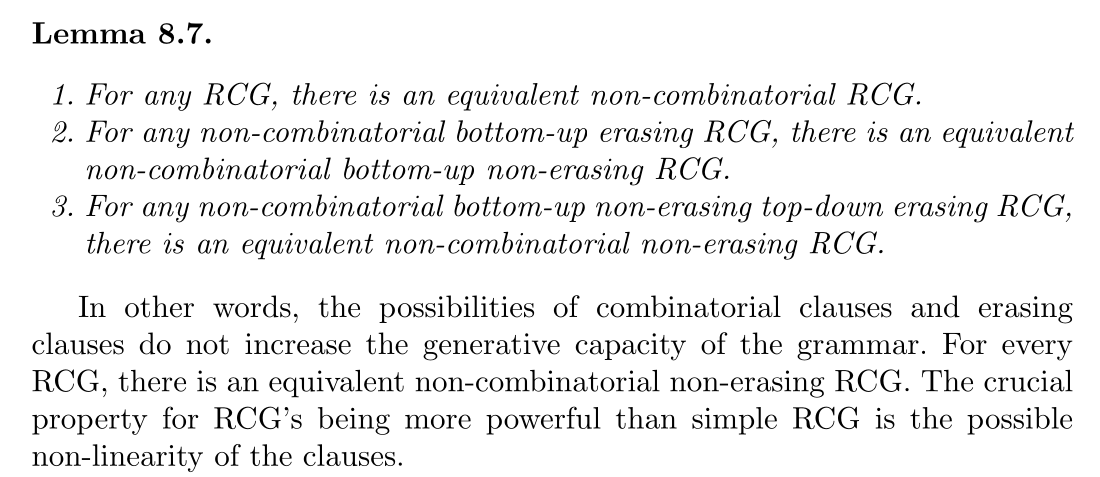
\includegraphics[width=0.88\textwidth]{../media/oponencia-3.png}\\[0.4em]
    {\scriptsize Kallmeyer (2010), \emph{Parsing Beyond Context-Free Grammars}, Lemma 8.7, p.~163.}
  \end{center}
\end{frame}

\begin{frame}{Oponencia --- pregunta 3 (respuesta)}
  \textbf{¿Cuánto cuesta la transformación?}

  Boullier la da en tres pasos locales (Propiedades 1--3):
  \begin{itemize}
    \item<2-> No combinatoria: cada cláusula combinatoria $\to$ tres cláusulas.
    \item<3-> No borrante (lado derecho, bottom-up): el predicado izquierdo gana un argumento con esa variable.
    \item<4-> No borrante (lado izquierdo, top-down): se añade un predicado $\mathrm{Any}$ que acepta cualquier cadena.
  \end{itemize}

  \vspace{0.3em}
  {\scriptsize Boullier (1998), \emph{A Proposal for a Natural Language Processing Syntactic Backbone}, Properties 1--3, pp.~11--12.}
\end{frame}

\begin{frame}{Oponencia --- pregunta 3 (respuesta)}
  \textbf{Ejemplo 1: no combinatoria}

  Cláusula combinatoria ($XY$ no es una variable suelta):
  \[ A(X,Y) \to B(XY) \]

  \pause
  Se reemplaza por tres cláusulas con predicados nuevos $c, c'$:
  \begin{align*}
    A(W, X, Y) &\to c(W, X, Y, W) \\
    c(W, X, Y, U\,Z\,V) &\to c'(X, Y, Z)\; B(W, Z) \\
    c'(X, Y, XY) &\to \varepsilon
  \end{align*}

  \pause
  \azul{$c'(X,Y,XY)$ usa la no linealidad para pegar las piezas.}
\end{frame}

\begin{frame}{Oponencia --- pregunta 3 (respuesta)}
  \textbf{Ejemplo 2: borrado (lado derecho, bottom-up)}

  $Y$ aparece solo a la derecha:
  \[ A(X) \to B(X, Y) \]

  \pause
  Se le da a $A$ un argumento nuevo con $Y$:
  \[ A(Y, X) \to B(X, Y) \]

  \pause
  \azul{Ahora $Y$ está en ambos lados.}
\end{frame}

\begin{frame}{Oponencia --- pregunta 3 (respuesta)}
  \textbf{Ejemplo 3: borrado (lado izquierdo, top-down)}

  Cláusula borrante (la $Y$ solo está a la izquierda):
  \[ A(XY) \to B(X) \]

  \pause
  Se reescribe añadiendo $\mathrm{Any}(Y)$:
  \[ A(XY) \to B(X)\,\mathrm{Any}(Y) \]
  \[ \mathrm{Any}(aX)\to\mathrm{Any}(X), \qquad \mathrm{Any}(\varepsilon)\to\varepsilon \]
  \begin{center}{\small \destacar{($a$ es un terminal cualquiera)}}\end{center}

  \pause
  $\mathrm{Any}$ acepta cualquier cadena: $Y$ se consume sin restringir nada, mismo lenguaje.

  \pause
  \azul{Es el mismo $\mathrm{Any}$ que, al intersectar con $A$, se vuelve $\mathrm{Reach}$ (pregunta 2).}
\end{frame}

\begin{frame}{Oponencia --- pregunta 3 (respuesta)}
  \textbf{Por qué es polinomial}
  \begin{itemize}
    \item<1-> Propiedad 1: cada cláusula combinatoria da a lo sumo 3 (factor constante).
    \item<2-> Propiedad 2: sube la aridad, no el número de cláusulas.
    \item<3-> Propiedad 3: añade $\mathrm{Any}(Y)$ y un bloque fijo de $O(|T|)$ cláusulas.
    \item<4-> $G_{\mathrm{cons}}$ ya es no borrante y no combinatoria.
  \end{itemize}
\end{frame}

\begin{frame}{Oponencia --- pregunta 3 (respuesta)}
  \textbf{Por qué la igualdad de rangos basta}
  \begin{itemize}
    \item<1-> Una variable repetida es la misma pieza de $w$ en varios predicados.
    \item<2-> En el recorrido real, esa pieza se atraviesa una vez: un solo par de estados.
    \item<3-> \destacar{La condición obliga a que todas sus ocurrencias lleven ese par.}
    \item<4-> Sin ella, los índices describirían un recorrido falso, y $G'$ aceptaría cadenas fuera de la intersección.
  \end{itemize}
\end{frame}

\end{document}
